% chktex-file 12  interword spacing in captions is intentional
% chktex-file 24  \label on own line is standard practice
% chktex-file 38  American-style punctuation inside closing quotes is correct
\chapter{Structural Vulnerability in the DoD Semiconductor Value Chain}
\label{chap:network_analysis}

In a large-scale conflict, the Department of Defense's ability to generate, deploy, and sustain combat power is dependent on continuous access to semiconductors. Chips are not a niche input reserved for a handful of exquisite platforms; they pace repair cycles, gate replenishment, and condition the availability of communications, sensing, precision guidance, and mission computing. That dependence creates an operational vulnerability that an adversary can exploit without ever engaging U.S. forces directly: by disrupting key points in the semiconductor value chain, an adversary can deny access outright or delay it long enough to impose schedule slippage that degrades readiness, compresses options in crisis, and stretches campaign timelines. The strategic question, then, is not whether the DoD is semiconductor-dependent, but where that dependence is structurally concentrated and which disruptions would impose the greatest downstream harm.

This section answers a specific question: if a firm (or a dependency relationship involving a firm) in the DoD-linked semiconductor dependency graph is disrupted, how much DoD-relevant semiconductor support is lost or delayed as a consequence of network structure? Here, ``support'' refers to semiconductor-relevant suppliers that are reachable, as well as the dependency paths connecting them to DoD prime contractors. The estimand is structural severity (structural consequence), not disruption probability. The analysis does not model who is likely to attack, when shocks will occur, or how frequently hazards materialize. Instead, the Section~\ref{chap:dod-supply-chain} graph is treated as a locked analysis object, and counterfactual disruption experiments on that object: nodes (firms) are removed from a directed dependency network that links semiconductor-relevant firms to DoD primes, and the resulting loss of reachability, fragmentation, and reduced redundancy (under a conservative proxy) is measured. Where useful, node removals are complemented with limited sensitivity checks on dependency ties, but the core approach is node-centered consequence measurement rather than edge-interdiction optimization.

The section presents three decision-relevant findings. First, targeted disruption is much more damaging than random failure. Removing a small number of structurally consequential firms results in a disproportionate loss relative to comparable random outages, indicating that continuity risk is shaped by identifiable leverage points rather than diffuse fragility. Second, vulnerabilities are concentrated on two attack surfaces. One is corridor intermediaries (nodes that mediate connections between semiconductor producers and prime contractors), which dominate prime-facing deny severity by severing many otherwise viable pathways between upstream capability and DoD endpoints. The other is upstream enablers to semiconductor firms---specialized providers whose position and scarcity make them consequential even when they are several steps removed from primes---especially under semiconductor-upstream targeting and delay-oriented objectives. Third, these results are translated into an actionable prioritization framework that combines measured impact with evidence confidence and semiconductor relevance, yielding a DoD-usable ``act now'' versus ``validate then act'' view. Heuristics and structural diagnostics help generate candidate sets, but the disruption experiments themselves establish severity.

Interpretation requires disciplined boundaries. Results are reported under three evidence-conditioned views of the same locked graph: disclosed, empirical (disclosed plus shipping), and augmented (empirical plus predicted). The analysis treats the empirical view as the decision-grade baseline because it combines disclosed relationships with independent flow evidence; the disclosed view is a conservative lower bound; and the augmented (full) view is a visibility-expanded sensitivity regime in which predicted links primarily function as prompts for validation and robustness checks, not as definitive proof of dependency. Finally, the outputs of this section are structural leverage points---not the most likely targets---and the analysis does not claim item-level provenance tracing of chips into specific weapons platforms. What it does provide is a rigorous, graph-based measure of continuity consequences in the DoD-linked semiconductor dependency environment, where disruption would be most harmful if it occurred.

%========================
% Section 4.1
%========================
\section{Analytic Framework}
\label{sec:ch4_framework}

This section evaluates structural severity, meaning the consequence for DoD-linked continuity in the fixed dependency network constructed in Section~\ref{chap:dod-supply-chain} when a firm becomes unavailable. Because the Section~\ref{chap:dod-supply-chain} graph is treated as locked, no new entity-resolution decisions are made, introduces no new edges, and does not expand the scope. The only variation arises from two deliberate choices: evidence-conditioned views of the same locked graph are evaluated, and, within each view, counterfactual disruptions and measures the resulting continuity outcomes on the same underlying structure. Consequence remains distinct from likelihood, so the analysis does not estimate hazard rates, intent, or targeting. It does not read high-severity positions as predictions about which firms will be disrupted \parencite{joint_task_force_transformation_initiative_guide_2012, kaplan_quantitative_1981}. Deny and delay serve as organizing language for the ways continuity can degrade under disruption, while remaining agnostic about why an outage occurs.

The analysis is organized around three operational questions. First, where would disruption impose the greatest deny-and-delay consequences for prime endpoints? Second, do those consequences concentrate among corridor intermediaries near primes or among upstream enablers of semiconductor firms? Third, which findings are robust to evidence uncertainty, and which should be treated as validation priorities rather than decision-ready chokepoints? Heuristics generate candidates; disruption experiments establish severity.

The analysis treats the network as a directed representation of dependency. A directed edge indicates that one firm provides inputs, services, or enabling capacity that another firm relies on (provider$\rightarrow$dependent), so disruption can propagate downstream along the direction of the ties. A directed path into a DoD prime, therefore, represents an upstream dependency chain that can transmit denial or delay consequences toward the DoD anchor. Throughout, ``tiers'' refers to graph distance from the DoD primes, not contractual tiering or a claim about item-level sourcing. This reading rule matters because the disruption experiments ask a structural question: if a node is removed, which primes lose upstream support entirely, and where do remaining dependency routes lengthen or break in ways that signal schedule pressure. With that dependency logic in place, the next step is to define ``semiconductor support'' within this DoD-linked dependency fabric.

``Semiconductor support'' specifies which continuity outcomes are evaluated in this section and where severe consequences arise within the broader DoD-linked dependency network. A fixed set of strict semiconductor firms from Section~\ref{chap:dod-supply-chain} serves as the source set for the support computations, so severity is evaluated in terms of how disruptions alter semiconductor-to-prime connectivity across the full locked dependency fabric. The disruption calculations are not restricted to paths that remain inside a ``semiconductor-only'' subgraph. Separately, a value-chain relevance lens is applied post hoc to interpret and report which high-impact disrupted nodes are semiconductor-plausible and to produce semantically defensible prioritization lists. The following formalizes the objective lenses that translate ``severity'' into deny-and-delay-oriented consequences.

The analysis evaluates continuity consequences through two complementary lenses that map onto DoD concerns about denial and delay. Under a deny lens, severity captures whether the disruption eliminates effective upstream support into a prime, producing hard losses in reachability within the dependency fabric. Under a delay lens, severity is captured by increased shortest-path distance from strict semiconductor source nodes to prime endpoints and by an increased share of semiconductor-to-prime connections that become disconnected, reflecting schedule pressure even when some support remains. A separate conservative proxy quantifies exposure to single-thread dependencies, in which disruption collapses redundancy even when some connectivity persists. These lenses also help distinguish where structural consequences tend to arise. In \S\ref{sec:ch4_vulnerability}--\S\ref{sec:ch4_upstream}, corridor intermediaries close to primes dominate prime-facing deny severity, while upstream enabling firms become more consequential under semiconductor-upstream targeting and delay-oriented objectives. The following defines the disruption operator that generates the counterfactuals used throughout the section.

The central analytic move in this section is counterfactual node removal. A firm is removed from the graph, along with its incident ties, and continuity outcomes are recomputed relative to the intact network. DoD agencies and prime contractors are treated as endpoints and are not removed in these experiments. This operator is intentionally broad. It captures a class of unavailability conditions---technical outages, financial failure, regulatory exclusion, or other interruptions---without requiring a model of which mechanism is more likely. While edge-level checks are, in principle, possible, they are limited, optional, and do not underpin the section's headline severity claims. Node removal as a robustness operator is well established in the network science literature, particularly for contrasting targeted disruptions with random failures \parencite{albert_error_2000,newman_networks_2018}. Because the same disruption can yield different conclusions depending on what evidence is included in the network, the following explains the section's evidence-conditioned graph views.

Interpretation depends on which evidence is admitted into the dependency fabric, so severity is reported under three evidence-conditioned views of the same locked graph. The disclosed view retains disclosed commercial relationships only. The empirical view adds observed shipping links and serves as the decision-grade baseline because it pairs disclosed ties with independent flow evidence. The augmented view adds predicted links to expand visibility, but those ties are treated as prompts for validation and robustness checks rather than definitive proof of dependency. Agreement between the empirical and augmented views increases confidence that a severity finding is not an artifact of limited visibility, whereas large shifts flag cases in which additional supplier discovery could materially change what appears most consequential. The following states the interpretive guardrails for reading structural leverage without sliding into likelihood or targeting claims.

Structural severity identifies leverage points conditional on disruption. The analysis does not interpret high-impact nodes as the most likely targets, and does not infer intent, timing, or frequency of hazards from network position. The evidence-conditioned views are therefore reading aids for uncertainty rather than competing ``truth'' claims. Findings that remain stable across disclosed, empirical, and augmented views are more decision-ready. In contrast, findings that move substantially when predicted links are admitted are better treated as prompts for validation. The output is a disciplined prioritization of where continuity consequences would be greatest in the event of an outage, not item-level provenance tracing to specific weapons platforms. The following turns to the two positional patterns that organize the concentration of severe consequences within this dependency fabric.

Two structurally distinct ways a disruption can matter in this network are distinguished. Corridor intermediaries are firms that sit on many dependency routes linking upstream semiconductor capability to DoD primes, so removing them can sever effective support even when upstream production exists elsewhere. Upstream enablers are firms that supply specialized inputs or services to semiconductor-relevant producers, so their removal can degrade the semiconductor ecosystem and reduce redundancy in ways that are more naturally expressed as delay and fragility rather than as an immediate cutoff at the prime. These categories serve as an interpretive lens---defined by graph position---rather than as a classification that drives the disruption math. This framing clarifies where continuity consequences concentrate as the analysis moves from definitions to disruption experiments.

The framework in this section is designed to support a defensible ordering of structural consequences while keeping uncertainty explicit. Three attributes are therefore carried forward into the results: measured impact under counterfactual removals, evidence confidence based on cross-view stability, and a value-chain relevance lens to interpret and report which high-impact nodes are semiconductor-plausible. The empirical view anchors ``act now'' candidates because it is grounded in disclosed relationships and observed shipping. In contrast, the augmented view helps identify cases in which additional validation could change prioritization. This structure keeps the section's headline claims tied to node-centered consequence measurement, preventing predicted-sensitive findings from being mistaken for confirmed dependencies. With the estimand, disruption operator, and evidence regimes defined, the next sections implement the disruption experiments and report where severity is structurally concentrated.

%========================
% Section 4.2
%========================
\section{Structural Severity}
\label{sec:ch4_severity}

This section reports the first core empirical result. The DoD-linked semiconductor dependency network is comparatively resilient to random outages but highly sensitive to targeted disruption. With the empirical view as the baseline, the analysis compares the severity loss under random node removals to the loss under two targeted strategies---PageRank and corridor-bottleneck---summarized in Figure~\ref{fig:ch4_robustness_empirical}.

This robustness comparison distinguishes diffuse fragility from concentrated structural leverage. If continuity risk were broadly distributed, random removals and targeted removals of the same size would produce similar deny losses. If leverage is concentrated, targeted removals should be more damaging. Figure~\ref{fig:ch4_robustness_empirical} shows the latter pattern. For the same disruption budget, targeted removals ranked by PageRank centrality and corridor-bottleneck position produce substantially larger losses in $H1_{\log}$ than the random baseline, where the random curve is the mean across 30 independent random removal draws and $H1_{\log}$ weights each prime by the log of its obligated dollars.

This comparison is implemented using the empirical-evidence view of the locked dependency graph, which admits disclosed SCR ties and observed shipping links and treats DoD Tier-1 primes as fixed endpoints. Each disruption is modeled as the removal of a node. When a firm is removed, it is deleted from the graph along with its incident dependency ties, and the severity is recomputed on the modified network relative to the intact baseline. Removal budgets are defined over an eligible pool of removable firms. Specifically, the x-axis in Figure~\ref{fig:ch4_robustness_empirical} is the share of non-endpoint firms removed from that pool, not the share of all nodes in the graph. This design keeps the comparison disciplined. It holds the DoD anchors constant, applies identical budget fractions across random and targeted conditions, and attributes differences in severity to which firms are removed rather than to changes in what counts as removable.

The primary outcome in this section is deny severity, measured by $H1_{\log}$, defined as a log-obligation-weighted ``any-support'' reachability loss from the strict semiconductor source set to DoD primes. The source set is the fixed list of strict semiconductor firms from Section~\ref{chap:dod-supply-chain}, and DoD Tier-1 primes are the endpoints. For each prime, support is scored as a binary condition: the prime is treated as supported if at least one strict semiconductor firm can still reach it through a directed dependency path in the post-removal graph, and unsupported otherwise. These prime-level support indicators are then aggregated using weights based on the log of each prime's obligated dollars. In effect, this weighting gives more influence to primes with larger procurement exposure while tempering the extent to which a handful of extremely large primes dominate the metric. The y-axis in Figure~\ref{fig:ch4_robustness_empirical} reports the percent loss in this weighted any-support measure relative to the intact empirical-view network, plotted as $100\times H1_{\log}$.

% ----- Figure 4.1: Robustness under random vs. targeted node removal --------
\begin{figure}[tbp]
  \centering
  \caption[\textit{Robustness under random vs.\ targeted disruption (empirical view)}]
  {\textit{Robustness under random vs.\ targeted disruption (empirical view)}}
  \label{fig:ch4_robustness_empirical}

  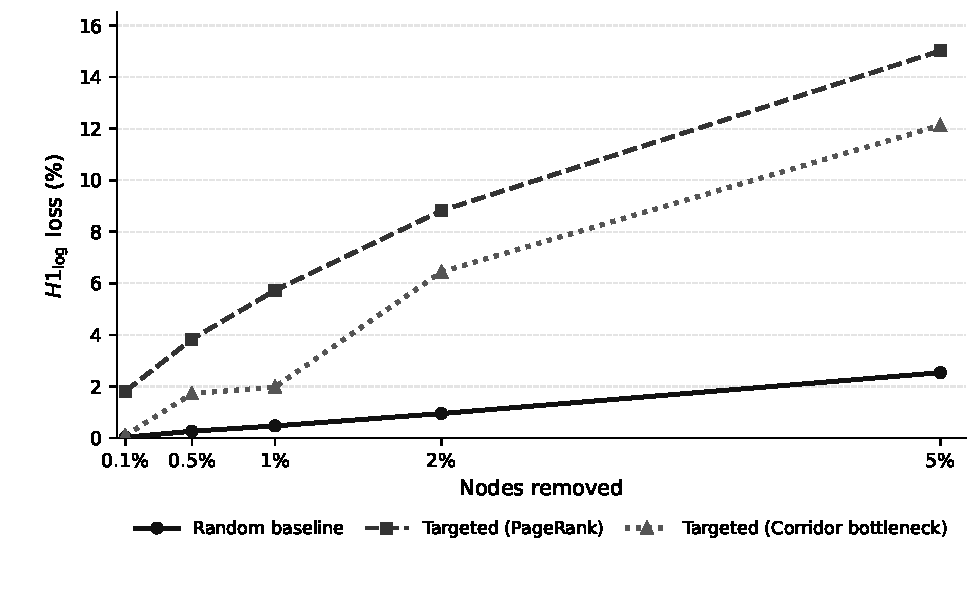
\includegraphics[width=\linewidth]{report/figures/fig_4.1_robustness_observed.pdf}

  \captionsetup{justification=raggedright,singlelinecheck=false}
  \caption*{\footnotesize \textit{Note}. This figure plots the percent loss in deny severity, $H1_{\log}$ ($100\times H1_{\log}$), as a function of the share of eligible removable non-endpoint firms removed. Results are computed on the empirical evidence view (disclosed SCR ties plus observed shipping), with DoD Tier-1 primes as endpoints. The random baseline reports the mean across 30 Monte Carlo node-removal draws at each removal fraction. Targeted removals are deterministic and rank nodes by PageRank centrality and corridor-bottleneck targeting (nodes that concentrate empirically supported semi$\rightarrow$prime corridor connectivity). Targeted disruption produces substantially larger losses than random removal at the same budget, consistent with a robust-yet-fragile structure. This motivates the budget-$k$ interdiction analysis in \S\ref{sec:ch4_budget_k} and the prioritization outputs in \S\ref{sec:ch4_decision}.}
\end{figure}

The random baseline serves as a benchmark for non-strategic outages. At each removal budget, that share of firms is randomly sampled from the eligible non-endpoint pool, removed, and $H1_{\log}$ is recomputed on the modified network. Because a single random draw can be idiosyncratic, the procedure is repeated 30 times for each budget, and the mean loss is reported. This Monte Carlo average provides the expected deny-severity loss when disruptions are not preferentially aimed at structurally important positions. Across the evaluated budget range, the random baseline increases gradually, indicating that most random firm outages produce only modest reductions in log-obligation-weighted any-support reaching DoD primes.

This random baseline is then compared to two targeted disruption strategies that remove firms chosen for structural importance rather than at random. The first targets firms ranked by PageRank centrality \parencite{Page1999}, a recursive measure that assigns higher importance to nodes connected to other important nodes in the directed dependency fabric. The second targets firms ranked by a corridor-bottleneck score that prioritizes corridor-intermediary positions, as defined in \S\ref{sec:ch4_framework}, i.e., firms that exhibit empirically supported connectivity between strict semiconductor sources and prime endpoints. In both cases, scores are computed once on the intact empirical-view graph and held fixed. For each budget, the top-ranked firms up to that budget are removed, without recomputing ranks after each removal. This fixed-order targeting design is sufficient to demonstrate concentrated leverage, even though adaptive re-ranking could change the magnitude of losses.

Appendix~\ref{app:c1_cross_view_stability} and Appendix~\ref{app:c2_stability_confidence_diagnostics} document cross-view stability and confidence diagnostics that support the section's uncertainty-conditioning framework. In the empirical-view experiment here, all strategies draw from the same eligible pool and budgets, so the targeted-versus-random separation is not an artifact of preselection.

This design keeps the random and targeted conditions directly comparable. All strategies draw removals from the same eligible non-endpoint firm pool and use the same budget fractions, so each condition removes the same number of firms at a given budget. The only difference is the selection rule. Random removals are evaluated by repeated sampling and averaged over draws, whereas the fixed baseline rankings fully determine the targeted removals. As a result, gaps between the random and targeted outcomes reflect the concentration of structural leverage in the network rather than differences in eligibility, endpoints, or how disruption budgets are defined.

The robustness curves show a large separation between random failure and targeted disruption across the evaluated budget range. When 1\% of eligible non-endpoint firms are removed, the random baseline yields a 0.5\% loss in $H1_{\log}$, while PageRank targeting yields a 5.7\% loss and corridor-bottleneck targeting yields a 2.0\% loss. At a 2\% budget, the random baseline is 0.9\%, compared to 8.8\% under PageRank targeting and 6.4\% under corridor-bottleneck targeting. At a 5\% budget, the random baseline reaches 2.5\%, while PageRank targeting reaches 15.0\% and corridor-bottleneck targeting reaches 12.1\%. In absolute terms, PageRank targeting adds 5.2 to 12.5 percentage points of additional deny loss relative to random at these budgets, while corridor-bottleneck targeting adds 1.5 to 9.6 percentage points. In relative terms, PageRank targeting produces roughly 6$\times$ the random loss at 5\% and about 9$\times$ at 2\%, while corridor-bottleneck targeting produces roughly 5$\times$ at 5\% and about 7$\times$ at 2\%.

These results establish that deny severity in the DoD-linked semiconductor dependency network is shaped by concentrated structural leverage rather than diffuse fragility. The remainder of the section, therefore, shifts from demonstrating the targeted-versus-random gap to locating where that leverage resides and how it should be prioritized under evidence uncertainty. \S\ref{sec:ch4_vulnerability} decomposes the high-impact set to distinguish corridor intermediaries near prime endpoints from upstream enabling firms that matter for semiconductor-side support. \S\ref{sec:ch4_budget_k} then turns to budget-$k$ disruption sets and contrasts deny- and delay-oriented objectives. \S\ref{sec:ch4_upstream} evaluates the second attack surface upstream of semiconductor firms, and \S\ref{sec:ch4_decision} translates the combined results into the decision layer. Appendix~\ref{app:c1_cross_view_stability} documents the cross-view stability and confidence diagnostics that underpin the section's uncertainty-conditioning framework and the confidence labels used later, including where the high-impact set is stable across empirically grounded evidence and where rankings become predicted-sensitive under visibility expansion.

%========================
% Section 4.3
%========================
\section{Where Vulnerability Lives}
\label{sec:ch4_vulnerability}

\S\ref{sec:ch4_severity} shows that targeted disruption is far more damaging than random outages in the empirical view. This section asks where that leverage sits within the DoD-linked dependency fabric and what kind of position yields the greatest prime-facing deny harm. The focus remains on deny severity, measured by $H1_{\log}$, with the empirical view as the decision baseline. The answer is summarized in two steps. First, the most damaging single-firm removals are identified by their location relative to primes. Second, a test examines how much of the top-$k$ deny harm can be recovered when the disruption set is restricted to specific positional cohorts at $k=25$, shown in Figure~\ref{fig:ch4_mechanism_decomposition}.

Vulnerability is located using two simple coordinates. The first is the distance to the primes. ``Tiers'' refers to the length of the shortest directed dependency chain from a firm to any DoD Tier-1 prime. This is graph distance, not contractual tiering. The second coordinate indicates whether a firm lies within the semiconductor$\rightarrow$prime corridor. The corridor is the set of firms that lie on at least one directed path from the strict semiconductor source set to DoD primes in the empirical view. Figure~\ref{fig:ch4_schematic_corridor_vs_upstream} provides a visual reference. Within the corridor, firms that are one step upstream of primes (prime-adjacent) are distinguished from other corridor intermediaries that still mediate connectivity into the prime endpoints. For the cohort comparisons below, a deeper-upstream tier region, referred to as ``upstream of semis,'' is also distinguished.

% ---------- Figure 4.2: Schematic corridor vs upstream ----------
\begin{figure}[tbp]
  \centering
  \caption[\textit{Semiconductor$\rightarrow$prime corridor schematic}]
  {\textit{Semiconductor$\rightarrow$prime corridor schematic}}
  \label{fig:ch4_schematic_corridor_vs_upstream}

  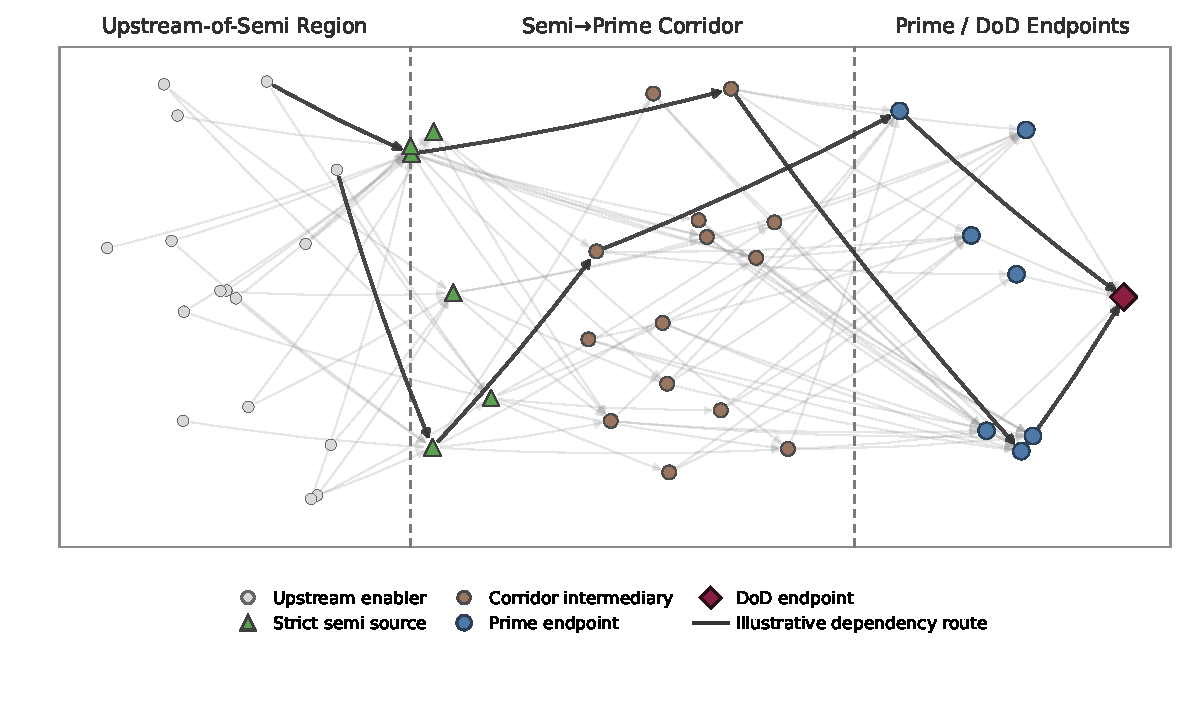
\includegraphics[width=\linewidth]{report/figures/fig_4.2_schematic_corridor_vs_upstream.pdf}

  \captionsetup{justification=raggedright,singlelinecheck=false}
  \caption*{\footnotesize \textit{Note}. This schematic provides a visual reference for the positional cohort logic used in Section~\ref{chap:network_analysis}. Dashed vertical boundaries partition a stylized directed dependency graph into three regions: an \textit{Upstream-of-Semi} region (left), the \textit{Semi$\rightarrow$Prime Corridor} (center), and \textit{Prime / DoD Endpoints} (right). Arrows indicate the direction of dependencies from upstream suppliers to downstream customers. Gray circles represent firms in the upstream-of-semis region, located several dependency steps upstream of primes and distinct from corridor intermediaries. Green triangles denote strict semiconductor source firms. Brown circles (\textit{corridor intermediaries}) represent non-endpoint firms that mediate connectivity from strict semiconductor sources into DoD Tier-1 prime endpoints (blue circles) under the section's empirical evidence view (disclosed SCR ties plus observed shipping). The red diamond denotes a DoD endpoint. The bold black polyline highlights an illustrative dependency route; faint edges indicate the surrounding context. For interpretive consistency with Figure~\ref{fig:ch4_mechanism_decomposition}, note that the corridor region contains both prime-adjacent nodes (one step upstream of primes) and other corridor intermediaries; prime-adjacent corridor nodes are visually marked as a corridor subset. The figure is illustrative (not a sampled subgraph and not to scale) and is intended to make the corridor mechanism, rather than node or edge counts, visually concrete.}
\end{figure}

For the comparisons in this section, firms are grouped into three positional cohorts relative to the semiconductor$\rightarrow$prime corridor. Prime-adjacent firms are one step upstream of DoD Tier-1 primes in the dependency reading. Corridor intermediaries sit inside the corridor but are not prime-adjacent. They mediate connectivity from strict semiconductor sources to the prime endpoints. Upstream of semis captures the semiconductor-side and deeper-upstream region of the graph. These firms sit beyond the prime-adjacent band and are not corridor intermediaries. This upstream region is separated because it represents a distinct way in which continuity can fail. Corridor intermediaries cut off prime-facing support by breaking the conduit into primes. Upstream disruptions can degrade the semiconductor side of the system even when corridor routes still exist.

A simple ranking exercise begins the analysis. In the empirical view, each eligible non-endpoint firm is removed one at a time, and the severity, $H1_{\log}$, is recomputed. This yields a single-firm impact score that answers a basic question: if this one firm were unavailable, how much prime-facing semiconductor support would be lost? The worst impacts are tightly clustered by position. Among the 25 most damaging single-firm removals, 24 are corridor intermediaries, and one is prime-adjacent. None is in the upstream-of-semis region. All 25 sit in the tier~2--3 band, meaning they lie within a couple of dependency links of a DoD prime.

This concentration pattern points to a specific mechanism. Tier~2--3 corridor intermediaries are not important because they are ``near'' primes in an abstract sense. They matter because they lie along many of the routes by which strict semiconductor capability reaches the prime endpoints. When one of these intermediaries is removed, multiple semiconductor$\rightarrow$prime support paths disappear at once. In effect, the corridor narrows. Upstream semiconductor production may still exist elsewhere in the graph, but it can no longer reach the primes through the remaining dependency fabric.

Figure~\ref{fig:ch4_mechanism_decomposition} tests this corridor mechanism directly. A disruption budget of $k=25$ is fixed in the empirical view, and the question is how much harm can be denied when the 25 removals must be made from a single positional cohort at a time. For each cohort, the 25 firms with the largest single-firm deny impacts are selected, and the resulting $H1_{\log}$ loss is evaluated. That loss is then scaled by the unrestricted deny comparator at the same budget. Corridor intermediaries recover \CorridorRecovery\% of the benchmark deny harm at $k=25$. Prime-adjacent targets recover 24.2\%. Upstream-of-semis targets recover 1.2\%. These percentages do not sum to 100 because each cohort is evaluated separately against the same unrestricted benchmark at $k=25$.

% ---------- Figure 4.3: Mechanism decomposition ----------
\begin{figure}[tbp]
  \centering
  \caption[\textit{Where deny vulnerability concentrates: cohort-constrained interdiction}]
  {\textit{Where deny vulnerability concentrates: cohort-constrained interdiction}}
  \label{fig:ch4_mechanism_decomposition}

  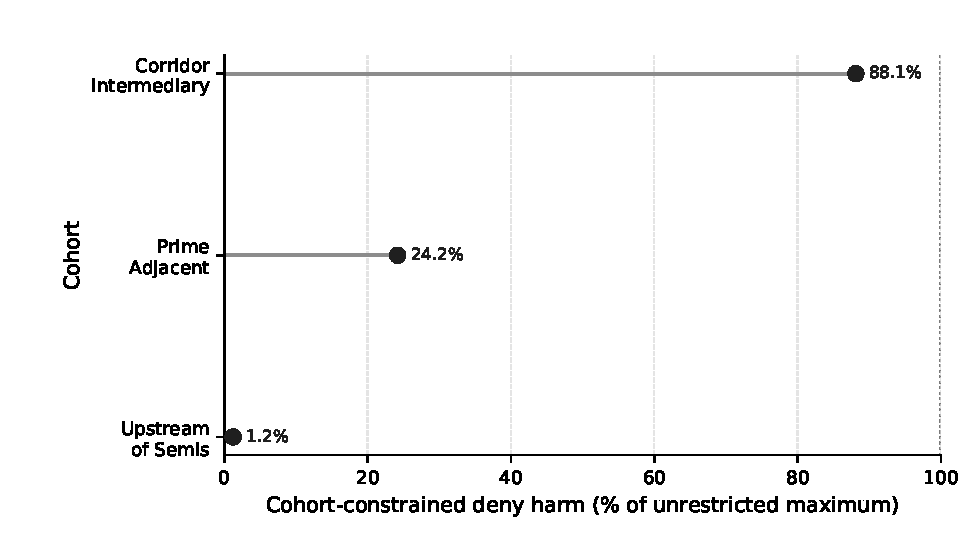
\includegraphics[width=\linewidth]{report/figures/fig_4.3_mechanism_decomposition.pdf}

  \captionsetup{justification=raggedright,singlelinecheck=false}
  \caption*{\footnotesize \textit{Note}. This figure reports cohort-constrained deny performance under the empirical evidence view (disclosed SCR ties plus observed shipping), with DoD Tier-1 primes as endpoints. For a fixed budget $k=25$, candidates within each cohort are ranked by their single-firm deny impact ($H1_{\log}$), and the top-$k$ prefix set is evaluated. Each point reports the resulting $H1_{\log}$ loss as a percentage of the unrestricted deny comparator at the same $k$. Values, therefore, do not sum to 100 across cohorts. Cohorts are defined by position relative to the empirically supported semiconductor$\rightarrow$prime corridor. \textit{Prime Adjacent} nodes sit one step upstream of primes. \textit{Corridor Intermediary} nodes lie in the corridor but are not prime-adjacent. \textit{Upstream of Semis} refers to firms deeper upstream in the tier partition, beyond the prime-adjacent band and outside the corridor-intermediary set. Corridor intermediaries recover \CorridorRecovery\% of the benchmark deny-harm at $k=25$, compared with 24.2\% for prime-adjacent and 1.2\% for upstream-of-semis targets.}
\end{figure}

The implication is that prime-facing deny vulnerability is mostly a corridor-intermediary problem in the empirical baseline. Restricting attention to corridor intermediaries retains nearly all of the harm achievable under an unrestricted budget. Restricting attention to prime-adjacent firms does not. Neither does restricting attention to the upstream-of-semis region. This does not mean upstream positions are irrelevant. This means that, under a prime-facing deny objective, the most damaging outages are those that break the conduit connecting semiconductor sources to the primes.

The concentration results in this section are reported under the empirical evidence view because they combine disclosed relationships with observed shipping evidence. The disclosed view is a lower bound because it omits shipping and may miss support routes present in the dependency fabric. The augmented view adds predicted links to expand visibility and is therefore treated as a sensitivity regime rather than a decision baseline. Appendix~\ref{app:c2_stability_confidence_diagnostics} summarizes how rankings shift across views. The top tail is stable from disclosed to empirical (22 of the Top-25 overlap), but it changes materially when predicted links are admitted (only 3 of the empirical Top-25 remain in the augmented Top-25). These cross-view stability diagnostics are used later to separate findings that are more decision-ready from those that are better treated as validation priorities.

These results locate where prime-facing deny vulnerability concentrates in the empirical baseline. The most damaging single-firm outages sit in the tier~2--3 corridor, and restricting a $k=25$ disruption set to corridor intermediaries recovers most of the deny harm achievable under an unrestricted budget. The remaining question is practical. If only a small number of firms can be prioritized for mitigation or monitoring, which specific set should be chosen under a fixed budget? \S\ref{sec:ch4_budget_k} answers that question by constructing budget-$k$ interdiction sets and showing how the selected firms change when the objective shifts from deny to delay.

%========================
% Section 4.4
%========================
\section{Efficient Budget-\texorpdfstring{$k$}{k} Disruption Sets: Denial vs.\ Delay}
\label{sec:ch4_budget_k}

This section answers a constrained decision question implied by the prior results: given a fixed disruption budget $k$, which \emph{sets} of firm outages produce the greatest structural harm in the empirical evidence view (disclosed SCR ties plus observed shipping)? Two objective lenses capture distinct continuity failures. Under a \emph{deny} objective, severity is measured by $H1_{\log}$, the log-obligation-weighted loss of ``any-support'' connectivity from the strict semiconductor source set into DoD Tier-1 prime endpoints. Under a \emph{delay} objective, severity is measured by $H2$, the change in mean shortest-path length among still-connected semiconductor$\rightarrow$prime support paths relative to baseline, reported alongside a \emph{disconnect share} that captures the fraction of primes that lose all semiconductor support after removal. Table~\ref{tab:ch4_interdiction_performance_observed} summarizes how these objectives produce different high-leverage sets at $k\in\{5,10,25\}$. These budget levels span the policy-relevant scale from near-term targeted monitoring of a handful of critical nodes ($k=5$) through a moderate resilience agenda ($k=10$) to a broader assessment that tests whether harm continues to accumulate or plateaus as the budget grows ($k=25$).

The interdiction universe is defined in two layers. The removable universe is the full set of non-endpoint firms in the locked graph (DoD Tier-1 primes remain fixed endpoints and are never removed). However, the budget-$k$ interdiction search is not run over all removable firms directly. For tractability, the search is restricted to a screened shortlist of $n=100$ structurally plausible high-leverage firms constructed from the empirical evidence view, and objective-specific interdiction sets are then built from that shortlist. This constraint keeps the section focused on consequence measurement under a realistic selection budget, so the reported sets should be read as efficient \emph{within the screened search space}, not as globally optimal interdiction solutions.

The $n=100$ shortlist is constructed in two steps, with a greedy, stepwise selection rule applied within it. First, candidates flagged by multiple simple structural screens are pooled---screens that identify firms likely to mediate semiconductor$\rightarrow$prime dependency-signals tied to prime reachability, corridor-bottleneck position, and centrality/degree-style diagnostics. Second, this pooled candidate set is ranked by single-firm deny impact in the empirical view, and the top $n=100$ are retained as the interdiction shortlist. Within that shortlist, \emph{greedy} means stepwise and adaptive selection: starting from an empty set, at each step the remaining candidate that produces the largest additional increase in the chosen objective (deny via $H1_{\log}$ loss, or delay via $H2$ growth) is selected, outcomes are recomputed on the modified graph, and the process repeats until the budget $k$ is reached. Because the choice is made one step at a time within a screened space, these sets are best interpreted as a transparent heuristic approximation to ``efficient under constraints,'' not a guarantee of a global optimum.

Three continuity outcomes are computed for these budget-$k$ experiments: two deny variants and one delay metric. The headline deny objective is $H1_{\log}$, which weights prime-level ``any-support'' loss by the log of each prime's obligated dollars; in parallel, a unit-weighted deny variant that treats primes equally serves as a check that results are not an artifact of obligation weighting. The delay objective is $H2$, defined as the change in mean shortest-path length among still-connected semiconductor$\rightarrow$prime support paths relative to baseline, and a disconnect share is reported alongside it to capture the fraction of primes that lose all semiconductor support after removal. For clarity and to keep the main text focused, Table~\ref{tab:ch4_interdiction_performance_observed} reports the headline subset-deny via $H1_{\log}$ and delay via $H2$, with disconnect share shown for both objectives.

Because $H1_{\log}$ and $H2$ capture different failure modes, they are interpreted jointly. The deny metric, $H1_{\log}$, is an \emph{any-support} measure. For each DoD Tier-1 prime, whether at least one strict semiconductor source can still reach that prime through a directed dependency path after removals is recorded, and prime-level losses are aggregated using log-obligation weights. The delay metric, $H2$, is defined over the set of \emph{still-connected} semiconductor$\rightarrow$prime support paths, so it measures route stretching among surviving routes rather than total loss of connectivity. \emph{Disconnect share} is therefore reported alongside $H2$, defined as the fraction of primes that lose all semiconductor support after removal. When the disconnect share rises, $H2$ can move counterintuitively because longer, more indirect routes often break first, leaving a smaller set of shorter connected routes and lowering the mean path length among those that remain.

Table~\ref{tab:ch4_interdiction_performance_observed} summarizes the performance of the objective-specific greedy interdiction sets in the empirical evidence view at budgets $k\in\{5,10,25\}$. Read the table in two passes. First, read within each objective as $k$ increases to see how harm scales with budget. Under deny selection, $H1_{\log}$ loss rises from $0.0359$ to $0.1009$ as $k$ moves from 5 to 25, and disconnect share rises from $0.0158$ to $0.0454$. Under delay selection, $H2$ growth rises from $0.0200$ to $0.0532$, while disconnect share remains lower and rises from $0.0043$ to $0.0187$. Second, compare objectives for the same $k$ to assess the trade-off between cutting support and stretching remaining routes. At each budget, deny-optimized sets yield larger $H1_{\log}$ losses than delay-optimized sets, whereas delay-optimized sets yield positive $H2$ growth with fewer disconnections. The negative $H2$ values under deny are consistent with the interpretation in the prior paragraph, in which longer routes tend to disconnect first, and the mean path length among the remaining connected routes can fall even as overall harm increases.

% -------------- Table 4.1: Budget-k interdiction performance -----------------
\begin{table}[tbp]
  \centering
  \caption[\textit{Budget-$k$ interdiction performance (deny vs.\ delay)}]
  {\textit{Budget-$k$ interdiction performance (deny vs.\ delay).}}
  \label{tab:ch4_interdiction_performance_observed}

  \footnotesize
  \setlength{\tabcolsep}{6pt}
  \renewcommand{\arraystretch}{1.04}

  % =======================
% Table 4.1 (tabular only)
% Budget-k interdiction performance (Observed view)
% =======================
\begin{tabular*}{\textwidth}{@{\extracolsep{\fill}} l
  S[table-format=2.0]
  S[table-format=1.4]
  S[table-format=-1.4]
  S[table-format=1.4]@{}}
\toprule
Objective
& \multicolumn{1}{c}{$k$}
& \multicolumn{1}{c}{$H1_{\log}$ loss}
& \multicolumn{1}{c}{$H2$ growth}
& \multicolumn{1}{c}{Disconnect share} \\
\midrule
Deny ($H1$)  &  5 & 0.0359 & -0.0539 & 0.0158 \\
Deny ($H1$)  & 10 & 0.0579 & -0.0701 & 0.0253 \\
Deny ($H1$)  & 25 & 0.1009 & -0.0983 & 0.0454 \\
\addlinespace[2pt]
Delay ($H2$) &  5 & 0.0098 &  0.0200 & 0.0043 \\
Delay ($H2$) & 10 & 0.0168 &  0.0323 & 0.0074 \\
Delay ($H2$) & 25 & 0.0416 &  0.0532 & 0.0187 \\
\bottomrule
\end{tabular*}


  \captionsetup{justification=raggedright,singlelinecheck=false}
  \caption*{\footnotesize \textit{Note}. Results report greedy node-removal interdiction under the empirical evidence view (disclosed SCR ties plus observed shipping), evaluated at disruption budgets $k\in\{5,10,25\}$. For each objective, outcomes are computed after removing the objective-specific \emph{greedy} interdiction set of size $k$. \textit{Deny (H1)} selects nodes to maximize $H1_{\log}$ loss (log-obligation-weighted loss of semiconductor support reaching DoD Tier-1 prime endpoints). \textit{Delay (H2)} selects nodes to maximize $H2$ growth (change in mean shortest-path length among still-connected semi$\rightarrow$prime support paths relative to baseline). \textit{Disconnect share} is the fraction of primes that lose all semiconductor support after removal. Negative $H2$ growth under the deny objective reflects a composition effect: interdiction disconnects longer routes first, lowering the mean path length among the remaining connected routes.}
\end{table}

Under the deny objective, the greedy interdiction sets produce substantial any-support loss even at small budgets. In Table~\ref{tab:ch4_interdiction_performance_observed}, deny-optimized removal yields $H1_{\log}$ loss of $0.0359$ at $k=5$, $0.0579$ at $k=10$, and $0.1009$ at $k=25$. The gains are front-loaded. The first five removals account for about 36\% of the total deny loss achieved at $k=25$, and the first ten account for about 57\%. As $k$ increases, fragmentation rises in parallel. Disconnect share grows from $0.0158$ at $k=5$ to $0.0454$ at $k=25$, meaning an increasing fraction of primes lose all semiconductor support under deny-optimized disruption. Under the same budgets, $H2$ growth is negative (from $-0.0539$ to $-0.0983$), consistent with the interpretation above. The deny-optimized sets tend to sever longer, more indirect routes first, so the mean path length among the remaining connected routes can decrease even as overall continuity harm increases. This pattern aligns with the corridor-intermediary mechanism emphasized in \S\ref{sec:ch4_vulnerability}, in which high-leverage deny consequences concentrate in prime-facing corridor positions.

Under the delay objective, the greedy interdiction sets increase path-length pressure while keeping fragmentation comparatively limited. In Table~\ref{tab:ch4_interdiction_performance_observed}, delay-optimized removal yields $H2$ growth of $0.0200$ at $k=5$, $0.0323$ at $k=10$, and $0.0532$ at $k=25$. The gains are again front-loaded, with the first five removals accounting for about 38\% of the total $H2$ growth achieved at $k=25$, and the first ten accounting for about 61\%. Under the same budgets, the disconnect share remains lower than under deny selection, increasing from $0.0043$ at $k=5$ to $0.0187$ at $k=25$. These delay-optimized sets still impose some deny harm, but it is substantially smaller than under deny optimization at the same $k$, with $H1_{\log}$ loss of $0.0098$, $0.0168$, and $0.0416$ at $k=5,10,25$. The delay rows indicate that the delay objective tends to select positions that stretch surviving semiconductor$\rightarrow$prime support routes rather than maximizing immediate cutoff through fragmentation.

These contrasts show that deny and delay are not interchangeable objectives, even under the same budget and the same screened search space. At a given $k$, deny-optimized sets consistently trade toward cutoff, producing larger $H1_{\log}$ losses and higher disconnect shares than delay-optimized sets. Delay-optimized sets trade toward route stretching, producing positive $H2$ growth with less fragmentation. The sign flip in $H2$ under denial is the composition effect made visible. At $k=25$, deny selection reaches $H1_{\log}$ loss of $0.1009$ with $H2$ growth of $-0.0983$ and disconnect share of $0.0454$, while delay selection reaches $H2$ growth of $0.0532$ with disconnect share of $0.0187$ and a smaller $H1_{\log}$ loss of $0.0416$. Read in this way, Table~\ref{tab:ch4_interdiction_performance_observed} implies that a mitigation posture focused only on the prime-facing deny corridor identified in \S\ref{sec:ch4_vulnerability} will not automatically cover delay-relevant vulnerabilities, and that delay-oriented sets can matter even when their deny footprint is modest.

These budget-$k$ results establish a practical decision boundary. Even under a tractable screened search space, small sets of outages can produce disproportionate structural harm, and the set that is efficient for denial is not the same as the set that is efficient for delay. Before translating these impacts into an actionable chokepoint list, \S\ref{sec:ch4_upstream} evaluates the second attack surface upstream of semiconductor firms, testing how upstream-of-semis targeting performs under the deny-and-delay lenses. \S\ref{sec:ch4_decision} then translates the combined findings into the decision layer by combining measured impact with evidence confidence and semiconductor relevance.

%========================
% Section 4.5
%========================
\section{Upstream of Semis: The Second Attack Surface}
\label{sec:ch4_upstream}

This section introduces a complementary results lens for continuity risk. \S\ref{sec:ch4_severity}--\S\ref{sec:ch4_budget_k} show that prime-facing consequence is dominated by corridor positions in the empirical view and that the efficient disruption set depends on whether the objective is deny or delay (Table~\ref{tab:ch4_interdiction_performance_observed}). A different decision question arises here: what constitutes high leverage when disruption is evaluated against the semiconductor-side support ecosystem rather than only against support reaching DoD primes? The same locked graph and node-removal operator are retained, with only the outcome lens changed, using the corridor versus upstream partition in Figure~\ref{fig:ch4_schematic_corridor_vs_upstream} as a visual guide.

In this section, ``upstream of semis'' refers to the supplier-side dependency environment that strict semiconductor firms rely on. Earlier, ``upstream-of-semis'' served as a positional cohort defined by graph distance to DoD primes. Here, the term is anchored on semiconductors themselves. Strict semiconductor firms serve as the anchor set, and consequences are evaluated for non-semiconductor firms that provide reachable upstream support to that set under the same empirical evidence view. The graph remains locked, and disruptions remain node removals on that locked topology. This lens is not a replacement for the prime-facing estimand. It is a complementary way to expose leverage that appears as semiconductor-side degradation even when support to primes is not immediately cut off.

A bounded empirical fact from the prime-facing results motivates this shift. In the empirical view of prime-facing single-node impacts, upstream-of-semis is nearly absent in the top tail. Zero of the Top-25 and Top-100 impacts fall in the upstream-of-semis cohort, and only one of the Top-500 does. The cohort-constrained comparison tells the same story. When a $k=25$ disruption set is restricted to upstream-of-semis nodes, it recovers only 1.2\% of the unrestricted deny harm and 1.98\% of the unrestricted delay harm (Figure~\ref{fig:ch4_mechanism_decomposition}). Under a prime-facing any-support estimand, upstream matters mainly when it changes semiconductor$\rightarrow$prime connectivity. These patterns do not imply that the semiconductor support base is robust. They show that upstream vulnerability can be difficult to see when consequences are evaluated only at prime endpoints.

The analysis, therefore, evaluates semiconductor-side outcomes using a semiconductor-anchored disruption analysis. Strict semiconductor firms serve as the anchor set, and node removals are scored by their effect on the size and structure of the non-semiconductor support ecosystem that remains reachable upstream of those semiconductors in the empirical view. Three outcome families are reported. First, semi-side reach loss captures the reduction in aggregate reachability from strict semiconductors into their upstream support endpoints. Second, semi-side path growth and a semi-side disconnect share capture route stretching among still-connected upstream support paths and the share of support endpoints that transition from baseline-reachable to unreachable after removal. Third, direct-entry fragility quantifies the frequency with which semiconductors lose immediate non-semiconductor supplier entry points and the frequency with which remaining support collapses to a single thread. In the empirical baseline, the evaluated graph includes $n_{\text{semis}}=1{,}994$ strict semiconductor nodes and $n_{\text{support endpoints}}=64{,}722$ non-semiconductor support-endpoint firms, and the baseline mean upstream path length is 2.8395.

Targeted-versus-random comparisons under this semiconductor-side lens show concentrated leverage. At a small budget of 0.1\% of removable non-semiconductor support firms (65 firms), PageRank targeting yields a semi-side reach loss of 0.0805, compared to 0.00210 under random removal, a 38.3$\times$ gap. A semiconductor-anchored heuristic that weights firms by the baseline support they provide and discounts by their distance from semiconductors shows a smaller gap at the smallest budget. Still, it outperforms random at smaller budgets. At 0.5\% removal, it yields a reach loss of 0.0186 versus 0.00930 under random, about 2.00$\times$, and at 1\% removal, it yields 0.0452 versus 0.0192, about 2.35$\times$. Fragility shifts sharply as well. At 0.5\% removal, this depth-weighted targeting increases the share of semiconductors with no direct non-semiconductor supplier entry by 0.0712, compared to 0.00050 under random removal.

Fixed-budget disruption sets under the semiconductor-side lens exhibit objective-specific trade-offs that parallel \S\ref{sec:ch4_budget_k}. Using the same screened-shortlist and greedy selection approach, $k$-sized removal sets are constructed that are efficient for the semi-side reach loss relative to the semi-side route stretching. At $k=25$, a deny-oriented set maximizes semi-side reach loss, yielding a reach loss of 0.1136. Within the same set, path growth is comparatively small at 0.0112. Still, fragmentation rises, with a disconnect share of 0.0463, and direct-entry fragility increases, with the share of semiconductors that lose all direct non-semiconductor supplier entry rising by 0.0125. A delay-oriented set behaves differently. At $k=25$, it yields path growth of 0.0861 with a disconnect share of 0.0369, while imposing a smaller reach loss of 0.0613 and a smaller direct-entry loss of 0.0035. Under a semiconductor-side lens, the choice of objective determines whether disruption manifests as an immediate support loss or as fewer redundant routes, which is a direct structural analogue of route stretching and brittleness, even at the same disruption budget. In operational terms, the delay-oriented set preserves more nominal support but forces it onto longer, fewer redundant routes, compressing schedule margins even at the same disruption budget.

These results show why the semiconductor-side support ecosystem is a distinct attack surface even when prime-facing denial is corridor-dominant. Under prime-facing metrics, upstream disruption appears weak because many outages do not immediately prevent semiconductor support from reaching primes. Under the semiconductor-side lens, the same small targeted budgets rapidly shrink the reachable support base and collapse redundancy at the semiconductor layer. The most important implication is that delay can be induced without a clean cutoff. An adversary need not sever the conduit into primes to cause operational harm. It can instead introduce brittleness in the semiconductor support base, making replenishment slower and less resilient to follow-on shocks.

Where does this semiconductor-side leverage sit relative to DoD primes? When the semiconductor-side single-node impact ranks are mapped back onto the prime-distance strata used earlier, the top tail is concentrated near the corridor band rather than in deep upstream tiers. In the Top-100 semiconductor-side impacts, 55 nodes are corridor intermediaries and 45 are near-prime, with none in the deep upstream strata. The same pattern holds for the fixed-budget disruption sets. At $k=25$, both the deny-oriented and delay-oriented sets are composed entirely of near-prime and corridor-intermediary nodes, with 14 near-prime and 11 corridor-intermediary selections in each. This alignment matters for interpretation. In this DoD-anchored dependency fabric, the second attack surface is not primarily a distance-to-prime story. It is a semiconductor-side degradation channel that is often instantiated through firms that also sit in the corridor band.

\S\ref{sec:ch4_decision} returns to the section's decision layer, translating prime-facing structural consequences into reporting-grade chokepoints based on measured impact, evidence confidence, and semiconductor relevance. The results in this section serve a different purpose. They show that the semiconductor support base can become brittle under small, targeted disruptions, even when prime endpoints remain nominally supported, making delay and fragility a distinct planning problem alongside conduit-cutoff risk. Read together, the two attack surfaces imply a two-part posture. Corridor chokepoints anchor near-term continuity mitigation and monitoring for prime-facing denial, while semiconductor-side degradation motivates parallel validation and resilience work aimed at upstream support robustness. \S\ref{sec:ch4_synthesis} synthesizes how to use these outputs together, including when to act, when to validate, and how to interpret the remaining uncertainty.

%========================
% Section 4.6
%========================
\section{Decision Layer: Value-Chain Chokepoints}
\label{sec:ch4_decision}

This section provides the decision layer. The structural severity estimates from the empirical view are translated into a defensible set of semiconductor value-chain chokepoints for reporting and prioritization. This requires separating three ideas that are easy to conflate in a raw ranking. Impact is the measured consequence of removing a counterfactual node. Evidence confidence reflects the stability of a finding across disclosed, empirical, and augmented views. Semiconductor relevance is a post-analysis reporting constraint that distinguishes value-chain-plausible chokepoints from structurally consequential but semantically uncertain candidates. The resulting prioritization is summarized in an impact-by-confidence action matrix in Figure~\ref{fig:ch4_action_matrix}, and a strict, empirical Top-25 chokepoint shortlist is reported in Table~\ref{tab:ch4_strict_top25}.

A raw severity ranking is not yet a defensible list of semiconductor chokepoints. The structural estimand treats directed ties as evidence of dependence, but the underlying relationship semantics are broad and heterogeneous in their implications for operational reliance. As a result, a firm can be highly consequential within the dependency fabric while occupying an adjacent or ambiguous position in the semiconductor value chain. For decision reporting, the severity estimates are kept fixed, and a separate semiconductor-relevance lens governs which high-impact nodes are treated as value-chain chokepoints.

This relevance step is a reporting layer rather than a new analysis pass. The locked graph is unchanged, no edges are added, and no severity metric is recomputed. The impact values reported in this section are the same counterfactual single-node removal estimates used throughout the section. What changes is how the high-impact universe is presented and interpreted for decision use. Firms that are structurally consequential but semantically uncertain are retained and tracked as validation priorities, rather than promoted as confirmed value-chain chokepoints in the main text.

Semiconductor relevance is implemented with a simple, auditable coding rule based on industry classifications \parencite{factset_standard_2021}. For each firm, its RBICS and SIC codes are read and mapped to a pre-registered codebook of semiconductor value-chain roles. If the codes indicate direct participation in the semiconductor value chain---for example, chip design, wafer fabrication, materials, equipment, assembly, test, or packaging---the firm is classified into the strict value-chain stream. If the codes point to an adjacent sector or are too generic to interpret, the firm is flagged as uncertain. Uncertain cases are not promoted as headline chokepoints but are retained as validation priorities. When a firm has multiple candidate codes, deterministic precedence rules ensure the same inputs always produce the same classification, and a reason code records why the firm was treated as strict or uncertain.

Industry codes alone can be too coarse to justify calling a firm a semiconductor chokepoint, especially near primes, where many suppliers may appear similar on paper. An empirical corridor gate, therefore, ensures the codebook does not promote firms that are not actually part of any DoD semiconductor support route in the empirical network. A firm qualifies for the strict chokepoint stream only if it lies on at least one directed support path that starts at a strict semiconductor firm and ends at a DoD Tier-1 prime in the empirical view. That is, the firm must connect on both sides as part of a realized support route. Endpoint overrides ensure known anchors are treated consistently, even when their industry codes are generic.

This relevance procedure yields two reporting streams. The strict stream contains firms that map cleanly to a semiconductor value-chain role and satisfy the corridor gate, so they can be reported as value-chain-plausible chokepoints when they are also high-impact. The adjacent or uncertain stream contains firms that remain structurally consequential but are semantically ambiguous under industry codes or are not supported as value-chain chokepoints in the empirical network. The decision layer is intentionally conservative. Only high-impact nodes from the strict stream are promoted as audit-ready chokepoints in the main text, reported in Table~\ref{tab:ch4_strict_top25}. The adjacent or uncertain stream is retained as a structured validation queue and documented in Appendix~\ref{app:c3_adjacent_uncertain_validation} to preserve transparency about which high-impact nodes were not promoted and why.

With relevance enforced, a decision rule is still needed to separate findings that are stable under evidence uncertainty from those that are visibility-sensitive. Actionability is treated as the combination of impact, evidence confidence, and semiconductor relevance. Impact is the measured consequence of removing a node in the empirical view, summarized by the primary deny metric $H1_{\log}$. Evidence confidence is a cross-view stability signal based on whether a node continues to appear among high-impact candidates when the disclosed, empirical, and augmented views are compared. In implementation, Figure~\ref{fig:ch4_action_matrix} bins candidates by impact and confidence only, while semiconductor relevance is enforced through the strict stream used to construct the prioritized shortlist in Table~\ref{tab:ch4_strict_top25}.

Figure~\ref{fig:ch4_action_matrix} summarizes impact and evidence confidence. The matrix is constructed over a cross-view high-impact candidate universe, defined as the union of the per-view Top-$N$ lists (the pre-specified cross-view Top-$N$ union) from the single-node impact ranks in the disclosed, empirical, and augmented views. For each candidate, two quantities are tracked. The first is its best (lowest) rank across the three views under the primary deny impact ranking based on $H1_{\log}$. The second is its cross-view presence count, meaning the number of views in which it appears in the Top-$N$ universe. Nodes are then binned by impact and confidence. A node is classified as high impact if its best rank falls within the high-impact cutoff; otherwise, it is classified as low impact. A node is classified as high-confidence if it appears in at least two views; otherwise, it is classified as low-confidence.

% -------------- Fig 4.4 Action Matrix: Impact x Confidence -------------------
\begin{figure}[tbp]
  \centering
  \caption[\textit{Action matrix for prioritizing structural chokepoints}]{\textit{Action matrix for prioritizing structural chokepoints}}
  \label{fig:ch4_action_matrix}
  % Figure 4.4 Action Matrix (no fill, table-style headers; dissertation style)
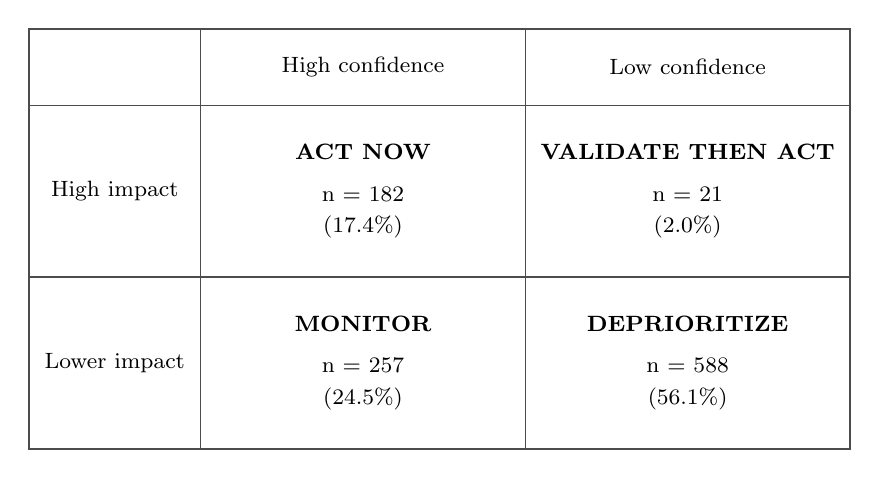
\begin{tikzpicture}

  % ---- sizing knobs ----
  \pgfmathsetlengthmacro{\AMcellw}{0.34*\linewidth}  % main cell width
  \pgfmathsetlengthmacro{\AMcellh}{0.18*\linewidth}  % main cell height
  \pgfmathsetlengthmacro{\AMhdrw}{0.18*\linewidth}   % left header column width
  \pgfmathsetlengthmacro{\AMhdrh}{0.08*\linewidth}   % top header row height

  % ---- derived geometry ----
  \pgfmathsetlengthmacro{\AMW}{\AMhdrw + 2*\AMcellw}
  \pgfmathsetlengthmacro{\AMH}{\AMhdrh + 2*\AMcellh}
  \pgfmathsetlengthmacro{\AMyMid}{\AMcellh}
  \pgfmathsetlengthmacro{\AMyTop}{2*\AMcellh}
  \pgfmathsetlengthmacro{\AMxLeft}{\AMhdrw}
  \pgfmathsetlengthmacro{\AMxMid}{\AMhdrw + \AMcellw}

  \definecolor{AMLine}{gray}{0.30}

  % ---- borders ----
  \draw[AMLine, line width=0.85pt] (0,0) rectangle (\AMW,\AMH);
  \draw[AMLine, line width=0.50pt] (\AMxLeft,0) -- (\AMxLeft,\AMH);
  \draw[AMLine, line width=0.50pt] (\AMxMid,0) -- (\AMxMid,\AMH);
  \draw[AMLine, line width=0.50pt] (0,\AMyMid) -- (\AMW,\AMyMid);
  \draw[AMLine, line width=0.50pt] (0,\AMyTop) -- (\AMW,\AMyTop);

  % ---- headers ----
  \node[align=center] at (\AMhdrw + 0.5*\AMcellw, \AMyTop + 0.5*\AMhdrh) {\footnotesize High confidence};
  \node[align=center] at (\AMhdrw + 1.5*\AMcellw, \AMyTop + 0.5*\AMhdrh) {\footnotesize Low confidence};

  \node[align=center] at (0.5*\AMhdrw, 1.5*\AMcellh) {\footnotesize High impact};
  \node[align=center] at (0.5*\AMhdrw, 0.5*\AMcellh) {\footnotesize Lower impact};

  % ---- cell text ----
  \tikzset{celltext/.style={align=center, inner sep=0pt}}

  % TOP-LEFT: ACT NOW
  \node[celltext] at (\AMhdrw + 0.5*\AMcellw, 1.5*\AMcellh) {%
    {\bfseries\footnotesize\scshape ACT NOW}\\[1.1mm]
    {\footnotesize n = 182}\\[-0.2mm]
    {\footnotesize (17.4\%)}%
  };

  % TOP-RIGHT: VALIDATE THEN ACT
  \node[celltext] at (\AMhdrw + 1.5*\AMcellw, 1.5*\AMcellh) {%
    {\bfseries\footnotesize\scshape VALIDATE THEN ACT}\\[1.1mm]
    {\footnotesize n = 21}\\[-0.2mm]
    {\footnotesize (2.0\%)}%
  };

  % BOTTOM-LEFT: MONITOR
  \node[celltext] at (\AMhdrw + 0.5*\AMcellw, 0.5*\AMcellh) {%
    {\bfseries\footnotesize\scshape MONITOR}\\[1.1mm]
    {\footnotesize n = 257}\\[-0.2mm]
    {\footnotesize (24.5\%)}%
  };

  % BOTTOM-RIGHT: DEPRIORITIZE
  \node[celltext] at (\AMhdrw + 1.5*\AMcellw, 0.5*\AMcellh) {%
    {\bfseries\footnotesize\scshape DEPRIORITIZE}\\[1.1mm]
    {\footnotesize n = 588}\\[-0.2mm]
    {\footnotesize (56.1\%)}%
  };

\end{tikzpicture}




  \captionsetup{justification=raggedright,singlelinecheck=false}
  \caption*{\footnotesize \textit{Note}. This matrix translates structural severity estimates into a decision-oriented triage for the locked graph using the disclosed, empirical, and augmented evidence views. Cells partition the cross-view high-impact candidate universe ($N=1{,}048$) by \textit{impact} (high vs. low) and \textit{evidence confidence} (high vs. low). Impact is based on the primary deny metric, $H1_{\log}$, which weights prime endpoints by log-obligations and measures the loss of semiconductor support under counterfactual removals. Evidence confidence reflects cross-view presence: low-confidence cases appear in only one view and are therefore more view-dependent. This matrix bins only impact and confidence. Semiconductor relevance is enforced downstream through the strict value-chain lens used to construct Table~\ref{tab:ch4_strict_top25}, while semantically uncertain candidates are tracked separately for validation in Appendix~\ref{app:c3_adjacent_uncertain_validation}.}
\end{figure}

Read Figure~\ref{fig:ch4_action_matrix} as a four-way triage for decision use. \textsc{Act now} denotes candidates that are high impact and high confidence. These are nodes whose removal yields a large deny severity and whose placement is supported by at least two evidence views, so the finding is not tied to a single visibility regime. \textsc{Validate then act} denotes candidates that are high impact but low confidence. These nodes appear severe in only one view, which often implies that their importance depends on view-specific routing that can change when additional evidence is admitted. For example, a firm may appear to control many semi$\rightarrow$prime routes in one view, but fall out of the high-impact set once shipping evidence or predicted links reveal alternative pathways. In these cases, the appropriate posture is to corroborate through targeted supplier discovery and adjudication before committing to mitigation. \textsc{Monitor} denotes candidates that are lower-impact but cross-view stable, making them persistent second-order leverage points worth tracking. \textsc{Deprioritize} denotes candidates that are both lower impact and view-dependent, where neither the estimated consequence nor the evidence warrants attention under a constrained decision budget. This matrix bins only impact and confidence. Semiconductor relevance is applied downstream, using the strict lens output to construct the chokepoint shortlist reported in Table~\ref{tab:ch4_strict_top25}.

% ---------- Table 4.2: Top-25 value-chain chokepoints ----------
\begin{table}[tbp]
  \centering
  \caption[\textit{Top-25 value-chain chokepoints}]{\textit{Top-25 value-chain chokepoints}}
  \label{tab:ch4_strict_top25}

  \footnotesize
  \setlength{\tabcolsep}{6pt}
  \renewcommand{\arraystretch}{1.04}

  % =======================
% Table 4.2 (tabular only, lean main-text)
% Strict observed Top-25 value-chain chokepoints
% =======================
\begin{tabularx}{\textwidth}{@{}c
  >{\hsize=1.0\hsize\raggedright\arraybackslash}X
  >{\hsize=1.0\hsize\raggedright\arraybackslash}X
  c
  S[table-format=1.4]@{}}
\toprule
Rank & Firm & Role & Corridor & {$H1_{\log}$} \\
\midrule
1  & TE Connectivity Plc & electronics interconnect & Near-prime & 0.0041 \\
2  & Comer Industries SpA & industrial components & Corridor & 0.0028 \\
3  & Aten International Co., Ltd. & electronics distribution & Corridor & 0.0026 \\
4  & Hurco Cos., Inc. & machine tools & Corridor & 0.0025 \\
5  & Hagener Feinstahl Bender & specialty metals & Corridor & 0.0024 \\
6  & George Risk Industries, Inc. & industrial controls & Corridor & 0.0023 \\
7  & Airgain, Inc. & RF components & Near-prime & 0.0021 \\
8  & Codan Ltd. & electronics systems & Corridor & 0.0021 \\
9  & D-Box Technologies, Inc. & electromechanical systems & Corridor & 0.0020 \\
10 & Velodyne Lidar, Inc. & sensing hardware & Near-prime & 0.0018 \\
11 & Aubert \& Duval SAS & specialty alloys & Corridor & 0.0017 \\
12 & Titomic Ltd. & advanced manufacturing & Corridor & 0.0016 \\
13 & Aspen Technology, Inc. & manufacturing software & Corridor & 0.0015 \\
14 & Arotech Corp. & defense electronics & Corridor & 0.0015 \\
15 & Quanta Computer, Inc. & EMS/ODM services & Corridor & 0.0014 \\
16 & Impinj, Inc. & semiconductor-enabled devices & Near-prime & 0.0014 \\
17 & Liebherr-International AG & industrial machinery & Corridor & 0.0013 \\
18 & ADTRAN Holdings, Inc. & communications hardware & Corridor & 0.0012 \\
19 & Metso Corp. & industrial equipment & Corridor & 0.0012 \\
20 & China International Marine & industrial manufacturing & Corridor & 0.0012 \\
21 & Vivotek Inc. & vision/security hardware & Corridor & 0.0012 \\
22 & D-Wave Quantum, Inc. & compute systems & Near-prime & 0.0012 \\
23 & Airbus SE & platform integrator & Corridor & 0.0011 \\
24 & Zhejiang Hailiang Co. Ltd. & primary metals & Corridor & 0.0011 \\
25 & Nordic Semiconductor ASA & fabless semiconductor & Near-prime & 0.0011 \\
\bottomrule
\end{tabularx}


  \captionsetup{justification=raggedright,singlelinecheck=false}
  \caption*{\footnotesize \textit{Note}. This table reports the 25 most structurally consequential nodes under the empirical view (including disclosed SCR ties and observed shipping) after applying the semiconductor value-chain strict relevance lens. Rows are ranked by $H1_{\log}$, the section's primary \textit{deny} severity metric. ``Corridor'' indicates nodes embedded in the empirically supported semi$\rightarrow$prime corridor. ``Near'' indicates nodes one step upstream of primes within that corridor definition. Role labels are interpretive and do not affect ranking.}
\end{table}

Table~\ref{tab:ch4_strict_top25} reports the semiconductor value-chain chokepoint shortlist sufficient for decision use. Figure~\ref{fig:ch4_action_matrix} is an impact and confidence triage over a cross-view high-impact universe, and it does not enforce semiconductor relevance. As a result, even candidates that fall in \textsc{Act now} can include firms that are structurally consequential but semantically adjacent to semiconductor continuity, such as generic enabling vendors that sit near primes. The strict relevance lens is therefore applied before promoting any firm as a semiconductor chokepoint. Table~\ref{tab:ch4_strict_top25} starts from the empirical-view single-node removal impacts, restricts the reporting universe to the strict value-chain stream produced by the codebook and corridor gate, and ranks rows by $H1_{\log}$, the log-obligation-weighted loss of semiconductor support to DoD Tier-1 prime endpoints under counterfactual single-node removal. The corridor label indicates whether a firm sits inside the empirically supported semi$\rightarrow$prime corridor and, when applicable, whether it is Near-prime or a corridor intermediary. Role labels summarize the mapped value-chain role and are interpretive. The confidence label in this table is specific to the strict Top-25 export. It is computed from cross-view presence within the strict Top-25 across disclosed, empirical, and augmented views and is reported as High, Medium, or Low. High-impact candidates that are structurally consequential but semantically uncertain are retained as a validation queue and documented separately in Appendix~\ref{app:c3_adjacent_uncertain_validation}.

To make the decision outputs concrete, the next step visualizes a representative local corridor neighborhood around a strict Top-25 chokepoint. It shows how single-node removal degrades prime-facing semiconductor support even when full disconnection is limited (Figure~\ref{fig:ch4_case_study_network_observed}).

Taken together, Figure~\ref{fig:ch4_action_matrix} and Table~\ref{tab:ch4_strict_top25} provide a conservative decision layer that keeps the estimand fixed while making uncertainty and semantics legible. The action matrix separates impact from stability, so high-impact, view-dependent cases are not mistaken for decision-ready chokepoints. The strict Top-25 table applies the semiconductor relevance lens to produce a semantically defensible shortlist for mitigation planning in the empirical baseline, while preserving a transparent record of excluded but consequential candidates in Appendix~\ref{app:c3_adjacent_uncertain_validation}. The next section grounds these decision outputs with an illustrative visualization and then documents robustness and interpretive limits.

%========================
% Section 4.7
%========================
\section{Robustness and Interpretive Limits}
\label{sec:ch4_robustness}

This section bounds how the decision outputs in \S\ref{sec:ch4_decision} should be interpreted under evidence uncertainty. The discussion first grounds the decision layer with an illustrative visualization that makes corridor degradation legible in the empirical view (Figure~\ref{fig:ch4_case_study_network_observed}), then summarizes the robustness and confidence diagnostics that support the uncertainty posture and states the key interpretive limits of the node-removal operator and the deny and delay metrics. The aim is to keep the results decision-useful without implying likelihood, intent, or item-level provenance.

Figure~\ref{fig:ch4_case_study_network_observed} provides a concrete view of what a high-impact chokepoint looks like inside the empirical dependency fabric. The focal node is selected from the strict empirical Top-25 list in Table~\ref{tab:ch4_strict_top25}, and a compact neighborhood is extracted using a deterministic corridor-based rule, so that the example is not hand-picked for effect. Panel~A shows the local subgraph under the empirical view before disruption. Panel~B shows the same node set under an identical layout after removing the focal node and its incident ties. The diagram is illustrative and local, not a rendering of the full Section~\ref{chap:network_analysis} network. Edges are shown without direction for readability.

% ---------- Figure 4.5: Illustrative local subgraph  ----------
\begin{figure}[tbp]
  \centering
  \caption[\textit{Illustrative local DoD-linked subgraph}]
  {\textit{Illustrative local DoD-linked subgraph}}
  \label{fig:ch4_case_study_network_observed}

  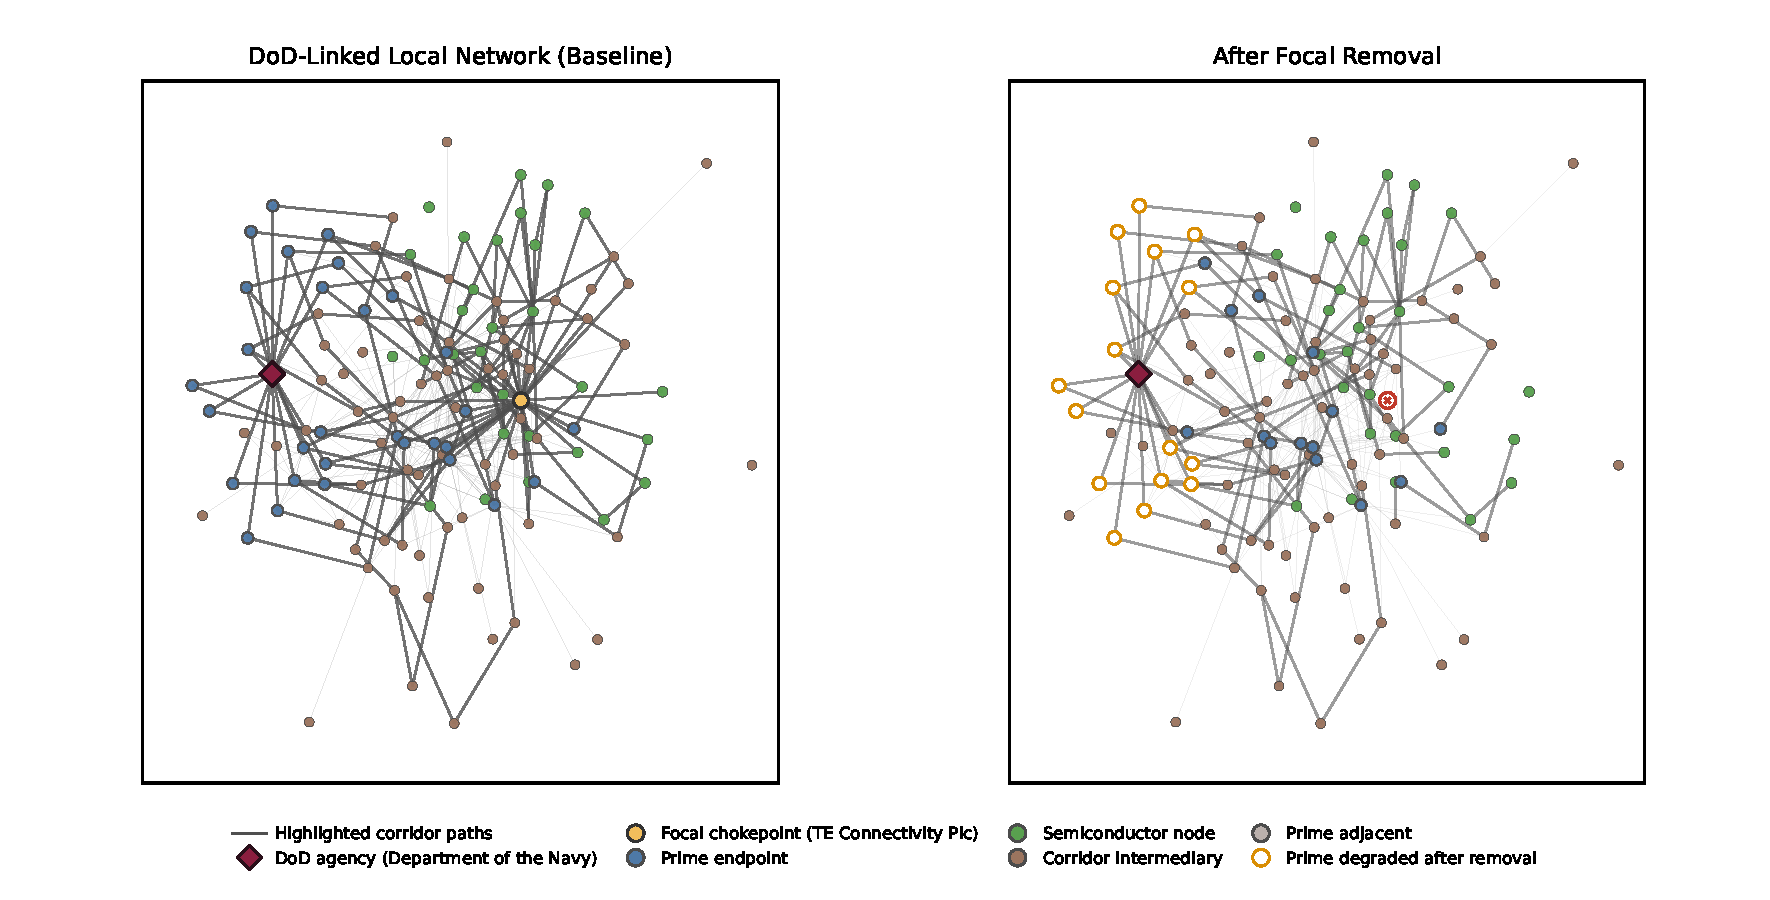
\includegraphics[width=\linewidth]{report/figures/fig_4.5_case_study_network_observed.pdf}

  \captionsetup{justification=raggedright,singlelinecheck=false}
  \caption*{\footnotesize \textit{Note}. This figure visualizes the mechanism quantified in Figures~\ref{fig:ch4_robustness_empirical} and~\ref{fig:ch4_mechanism_decomposition} and summarized in Tables~\ref{tab:ch4_interdiction_performance_observed} and~\ref{tab:ch4_strict_top25}. The diagram is an illustrative local subgraph extracted from the empirical evidence view (disclosed SCR ties plus observed shipping), not the full Section~\ref{chap:network_analysis} network. Panel~A shows a compact DoD-linked neighborhood anchored on the DoD Tier-0 component \textit{Department of the Navy} and centered on the focal chokepoint \textit{TE Connectivity}; Panel~B shows the same node set under an identical layout after removing the focal node and its incident edges (the red $\times$ marks its former location). Edges represent supply-like dependency ties and are rendered without direction for readability; darker edges highlight the corridor paths used to define the local corridor neighborhood, while lighter edges provide surrounding context. The rendered subgraph contains 130 nodes and 449 edges, including 18 strict semiconductor nodes and 16 selected prime endpoints. In this local neighborhood, focal removal fully disconnects 0 selected primes but degrades 16 (orange outlines): each remains reachable but with fewer supporting semiconductor paths and/or longer remaining shortest paths. Accordingly, the figure is intended to illustrate how single-node disruption can generate widespread \textit{delay/fragility} effects even when complete denial is limited in a given neighborhood.}
\end{figure}

After focal removal, most selected prime endpoints in this neighborhood remain reachable from at least one strict semiconductor source, but many are degraded. The degradation takes two forms. First, fewer distinct semiconductor-to-prime support paths remain, reducing redundancy and increasing exposure to additional shocks. Second, the remaining routes are often longer or more circuitous, which is consistent with the section's delay and fragility interpretation even when complete disconnection is limited in a given neighborhood. This visualization clarifies what the action matrix and the Top-25 shortlist summarize at scale. High impact reflects measured consequence under node removal, and the mechanism often operates through corridor narrowing and route degradation rather than immediate cutoff alone.

\S\ref{sec:ch4_framework} defines the three evidence-conditioned views. Here they serve as a robustness frame. The empirical view is treated as the decision-grade baseline, with disclosed and augmented as uncertainty-conditioning comparisons. Appendix~\ref{app:c1_cross_view_stability} and Appendix~\ref{app:c2_stability_confidence_diagnostics} audit how evidence admission changes top-tail membership and ordering under the same estimand and node-removal operator. In the augmented view, predicted links function as visibility-expansion prompts for validation rather than confirmed dependencies.

Appendix~\ref{app:c1_cross_view_stability} shows that admitting shipping evidence refines but does not rewrite the highest-impact tail. In the top 25, the disclosed and empirical sets share 22 overlapping nodes, and their ordering is highly consistent across the common ranked set. In contrast, overlap involving the augmented view is low at small $N$ and ordered agreement is weaker. This pattern is expected when predicted links expand feasible routing, thereby changing which nodes appear most consequential at the very top. It does not imply that the augmented view is inherently more trustworthy than the empirical baseline. The augmented view is treated as a sensitivity regime that flags where additional supplier discovery could plausibly change prioritization. For the full overlap curves and rank stability summaries across increasing Top-$N$ thresholds, see Figure~\ref{fig:app_c1_cross_view_overlap} and Table~\ref{tab:app_c1_crossview_stability_summary}.

Confidence appears in three places in this section, and the labels refer to cross-view stability rather than probability. In Figure~\ref{fig:ch4_action_matrix}, confidence is a binary presence screen used for triage. A candidate is classified as high confidence if it appears in the cross-view Top-$N$ universe in at least two views. In Appendix~\ref{app:c2_stability_confidence_diagnostics}, a three-tier version of the same idea is reported for the high-impact set, based on presence in three views, two views, or one view. In Table~\ref{tab:ch4_strict_top25}, a High, Medium, Low label computed within the strict Top-25 shortlist after applying the relevance lens is reported. These schemes are related, but they are not numerically interchangeable because they are computed over different candidate universes and serve different reporting purposes. In all cases, confidence is a guide for decision posture. It is not a probability of disruption, and it is not proof of any single supplier relationship.

Semantic uncertainty is handled through a conservative reporting rule rather than by discarding inconvenient cases. The strict Top-25 shortlist in Table~\ref{tab:ch4_strict_top25} applies the semiconductor relevance lens before promoting any firm as a value-chain chokepoint. A concrete example from the empirical run is Microsoft Corp. In the adjacent/uncertain stream, Microsoft is structurally high-impact (rank 1 in that stream, with single-node deny impact $H1_{\log}=0.0093$) and sits inside the tier~2--3 corridor. It also passes the empirical two-sided corridor gate, meaning it lies on at least one empirical support route that connects a strict semiconductor source to a DoD Tier-1 prime. Passing this gate is necessary but not sufficient for strict value-chain promotion. The industry-code evidence must also map cleanly to a semiconductor value-chain role.

In this case, the relevance procedure records an uncertain classification under the codebook rules, so Microsoft is not promoted into the strict value-chain Top-25. This is not surprising for a large enterprise software and cloud services provider. Its industry codes primarily signal general IT and business enablement rather than a semiconductor value-chain role, so the observed corridor position could reflect prime operational dependence without being semiconductor-specific support. Instead, it is retained as a validation priority where the next step is to adjudicate whether the observed dependency reflects semiconductor-specific support or a general enterprise enablement relationship that is consequential for primes but not specific to semiconductor continuity. The specific industry-code triggers that produced the adjacent/uncertain classification are reported as ``Code basis'' in Appendix~\ref{app:c3_adjacent_uncertain_validation}. Appendix~\ref{app:c3_adjacent_uncertain_validation} documents these adjacent/uncertain high-impact cases and how they should be handled before they are treated as confirmed value-chain chokepoints.

Node removal and the section's severity metrics are intentionally conservative structural operators and have limits that matter for decision-making. Removing a firm represents generic unavailability and does not model inventories, substitution, rerouting through alternative suppliers, or recovery time. The deny metric, $H1_{\log}$, captures support loss under reachability and should be read as a consequence measure conditional on outage rather than a forecast of realized disruption. The delay metric, $H2$, captures structural path-length pressure among surviving semiconductor-to-prime routes rather than calendar delay. It can also exhibit a compositional effect because longer routes often disconnect first, thereby lowering the mean path length among the routes that remain, even as overall harm increases. $H2$ is therefore interpreted jointly with disconnect share and with the qualitative mechanism in Figure~\ref{fig:ch4_case_study_network_observed}. Together, these caveats support a disciplined reading of the decision layer. The action matrix provides an impact and stability triage. Table~\ref{tab:ch4_strict_top25} provides a relevance-constrained shortlist for mitigation planning. Appendix~\ref{app:c3_adjacent_uncertain_validation} provides the validation queue for semantically ambiguous but structurally consequential cases.

With these guardrails in place, the section's results remain decision-useful without overclaiming. Stable, high-impact findings in the empirical baseline support near-term action on continuity risk reduction and monitoring, while view-dependent high-impact cases motivate targeted supplier discovery and traceability work before action. The strict Top-25 shortlist should be understood as a conservative set of value-chain-plausible chokepoints conditional on disruption, not as a claim about the most likely targets or the only relevant dependencies. One additional robustness dimension is deferred: temporal stability, which would test whether rankings shift materially under alternative graph-snapshot dates. Because that analysis requires additional historical graph builds beyond the current frozen snapshot, it is reserved for future work. \S\ref{sec:ch4_synthesis} synthesizes these findings and translates them into the section's final decision takeaways.

%========================
% Section 4.8
%========================
\section{Synthesis and Decision Use}
\label{sec:ch4_synthesis}

This section closes the analysis by making the results legible and actionable without requiring network-science fluency. It is intentionally not a recap of \S\ref{sec:ch4_severity}--\S\ref{sec:ch4_robustness}. Instead, the analysis is translated into a simple workflow that explains what the outputs mean in real operational terms. Figure~\ref{fig:ch4_action_matrix} presents the first filter, separating high-consequence findings that are stable across evidence views from those that are view-dependent and therefore require validation. Table~\ref{tab:ch4_strict_top25} then supplies the conservative starting shortlist of value-chain-plausible chokepoints in the empirical baseline for mitigation planning and monitoring. Appendix~\ref{app:c3_adjacent_uncertain_validation} records the cases that are structurally consequential but semantically uncertain and converts them into a disciplined validation queue rather than treating them as headline chokepoints.

The central question is how much semiconductor-relevant support DoD Tier-1 primes would lose or degrade, purely because of network structure, if any single firm in the DoD-linked dependency network were unavailable. The answer comes from a disciplined set of ``what if this firm goes offline'' stress tests on a locked dependency map. Holding the Section~\ref{chap:dod-supply-chain} object fixed, one firm at a time is removed, and how semiconductor support can still reach prime endpoints through the remaining network is recomputed. In real terms, the question is whether an outage collapses many routes at once, forces support onto fewer and more fragile detours, or eliminates all viable routes into a prime. Figure~\ref{fig:ch4_case_study_network_observed} provides a concrete illustration. Removing a single corridor node can degrade many endpoints at once, even when no endpoint is cleanly disconnected in that local view. The decision layer in Figure~\ref{fig:ch4_action_matrix} then translates these consequences into a posture for action versus validation under evidence uncertainty. Throughout, the posture is conditional. The analysis assesses the consequences if a disruption occurs, not who will be disrupted, when it will occur, or how likely any hazard is to materialize.

This decision translation carries through two failure modes that matter in practice: denial and delay. Denial is the hard case. A prime effectively loses semiconductor support because no viable support route remains from the strict semiconductor source set into that endpoint. Concretely, this appears to be a forced stop, an immediate scramble for substitutes, or a rapid drawdown of inventories while the program searches for an alternative qualified source. Delay is the softer but often more operationally plausible case. A prime is not fully cut off, but the remaining support routes become fewer, thinner, and more circuitous. In real terms, that means longer lead times, more handoffs across intermediate firms, less slack to absorb routine hiccups, and a higher chance that a follow-on disruption tips a merely degraded situation into outright denial. Figure~\ref{fig:ch4_case_study_network_observed} is the intuition anchor for this distinction. A single removal can leave endpoints nominally connected while degrading many of them at once by collapsing redundant routes and forcing the remaining routes onto longer or more brittle paths. That is also why delay severity is interpreted jointly with disconnect share in Table~\ref{tab:ch4_interdiction_performance_observed} rather than treating any one metric as a standalone statement about calendar time.

Figure~\ref{fig:ch4_action_matrix} is the first decision filter because it tests whether a high-consequence finding persists when the evidence admitted into the same locked network is varied. Read the matrix as triage under uncertainty. In the \textsc{Act now} cell, the result is both consequential and stable across evidence views, so it is less likely to be an artifact of missing visibility and more suitable to treat as a planning assumption. In the \textsc{Validate then act} cell, the result is consequential but view-dependent, which means it can be driven by a particular routing picture that changes once additional relationship evidence is admitted. Put differently, these are the cases in which the next step is not an immediate mitigation investment. The next step is to verify the actual dependency through supplier discovery and adjudication. Appendix~\ref{app:c1_cross_view_stability} and Appendix~\ref{app:c2_stability_confidence_diagnostics} provide the audit trail for this posture by showing how top-tail membership and ordering move across the disclosed, empirical, and augmented views.

Table~\ref{tab:ch4_strict_top25} is the conservative ``start here'' output for decision use. It is conservative in two ways. First, it is anchored on the empirical evidence view, which pairs disclosed relationships with observed shipping and serves as the section's decision-grade baseline. Second, it applies the strict semiconductor relevance lens before promoting any firm as a value-chain chokepoint. For a planner, this list is meant to support concrete continuity work. It identifies a small set of named firms for which an outage would impose disproportionate downstream consequences in this DoD-linked dependency environment, conditional on disruption. It is not a forecast of likely targets. It is not a complete inventory of all dependencies that matter to DoD mission performance. It is not item-level provenance tracing into specific platforms. The decision value is prioritization under constraint. If a planner can only monitor, engage, or harden a limited number of positions, Table~\ref{tab:ch4_strict_top25} provides the section's most defensible shortlist for the empirical baseline. At the same time, Figure~\ref{fig:ch4_action_matrix} preserves the broader triage context in which that shortlist sits.

Appendix~\ref{app:c3_adjacent_uncertain_validation} contains the cases that are structurally consequential in the dependency fabric but not yet defensible to label as semiconductor value-chain chokepoints. This queue prevents two common decision errors. The first is silently discarding high-impact findings because their industry codes look generic. The second is promoting them as ``semiconductor chokepoints'' when the evidence supports consequence but not value-chain role. A concrete example is the kind of enterprise software or cloud services provider that can sit close to primes and appear on important support routes. That position can be consequential for prime operations while remaining ambiguous as semiconductor-specific support. In the workflow implied by Figure~\ref{fig:ch4_action_matrix}, these cases belong in \textsc{Validate then act}. The immediate task is adjudication, not mitigation. Operationally, this means targeted supplier discovery, contract and dependency clarification, and traceability-oriented verification to determine whether the observed relationship reflects semiconductor-relevant enabling capacity or general enterprise enablement that should be handled through a different continuity lens.

The second attack surface in \S\ref{sec:ch4_upstream} changes how continuity planning should be conceived because it shows how harm can accumulate without a clean cutoff. Even when primes remain nominally supported, disruption can make the semiconductor production and replenishment base brittle by shrinking the upstream support ecosystem on which semiconductor firms rely, leaving fewer redundant routes. In real terms, this is the scenario where the system ``still works,'' but it works on fewer options, with less slack, and with more single points of failure outside the immediate prime-facing view. Lead times stretch, substitutions become harder to execute quickly, and routine perturbations that would normally be absorbed start to cascade as fewer redundant routes remain to carry the load. This does not overturn the corridor story. In this DoD-anchored object, semiconductor-side leverage largely maps back onto near-prime and corridor-adjacent positions rather than implying that distance-to-prime tiers dominate. The decision implication is therefore additive. Corridor chokepoints anchor efforts to prevent outright denial. At the same time, semiconductor-side brittleness poses a parallel planning problem, motivating validation and resilience efforts to reduce degradation and compounding-shock risk.

Taken together, the section's outputs support a simple decision workflow under constrained attention and imperfect visibility. The workflow starts with posture. The action matrix separates findings that are both consequential and stable from findings that are consequential but sensitive to what evidence is visible. Relevance discipline is then applied, so the result is not just a list of structurally important firms, but a defensible set of semiconductor value-chain chokepoints for reporting and mitigation planning. Finally, the remaining high-impact yet ambiguous cases are treated as a structured work plan for supplier discovery and adjudication rather than as noise. This workflow tells a decision-maker what to harden and monitor first, what to verify before committing resources, and what to treat as second-order but persistent leverage points. That translation from raw rankings to an ``act, validate, monitor'' posture is the primary decision output of this section.

Two extensions are reserved for the integrative discussion in Section~\ref{chap:from_illumination_to_assurance}. First, the corridor chokepoints identified here for continuity risk also represent high-leverage positions for integrity attacks---counterfeits, hardware Trojans, and toolchain tampering concentrate at the same structural bottlenecks---and the policy implications of that overlap are developed there. Second, the severity scores reported here measure structural consequence $S(n)$ only. Illustrative probability scenarios---for example, how the action-matrix priorities would shift if nodes in geopolitically exposed regions carry elevated disruption likelihood $P(n)$---require assumptions beyond the structural analysis and are explored in Section~\ref{chap:from_illumination_to_assurance} as part of the policy discussion.

Section~\ref{chap:from_illumination_to_assurance} shifts from measurement to policy design. Building on the decision workflow from Section~\ref{chap:network_analysis}, the identified high-consequence positions and the structured validation agenda are translated into a set of actionable policy and regulatory recommendations for the Department of Defense. The focus is on how DoD can reduce supply-chain opacity in ways that are realistic for acquisition and oversight, including traceability and provenance practices that make critical dependencies auditable across tiers and over time. The goal is not perfect transparency. It is decision-grade visibility that enables the DoD to verify the dependencies that matter, detect emerging chokepoints early, and make the semiconductor supply chain more defensible against denial and delay in a crisis.